\documentclass[letterpaper,12pt]{article}

%\usepackage{ucs}
%\usepackage[utf8x]{inputenc}
\usepackage{amsmath}
\usepackage{amsfonts}
\usepackage{amssymb}
%\usepackage[canadian]{babel}
\usepackage[margin=1in]{geometry}
\usepackage{graphicx}
\usepackage{hyperref}

\newcommand{\R}{\mathbb{R}}
\renewcommand{\i}{\mathbf{i}}
\renewcommand{\j}{\mathbf{j}}
\renewcommand{\k}{\mathbf{k}}

\newcommand{\bbm}{\begin{bmatrix}}
\newcommand{\ebm}{\end{bmatrix}}

\title{Solutions for Quiz 2 Practice Problems\\Math 2580\\Spring 2016}
\author{Sean Fitzpatrick}
%\date{January 14th, 2016}

\begin{document}
 \maketitle

If you can answer the following problems, you should be well-prepared for Quiz 2:

\begin{enumerate}
 \item Sketch the level curves $f(x,y)=c$ of the function $f(x,y)=x^2-y^2$, for $c=-2,-1,0,1,2$.

\begin{center}
 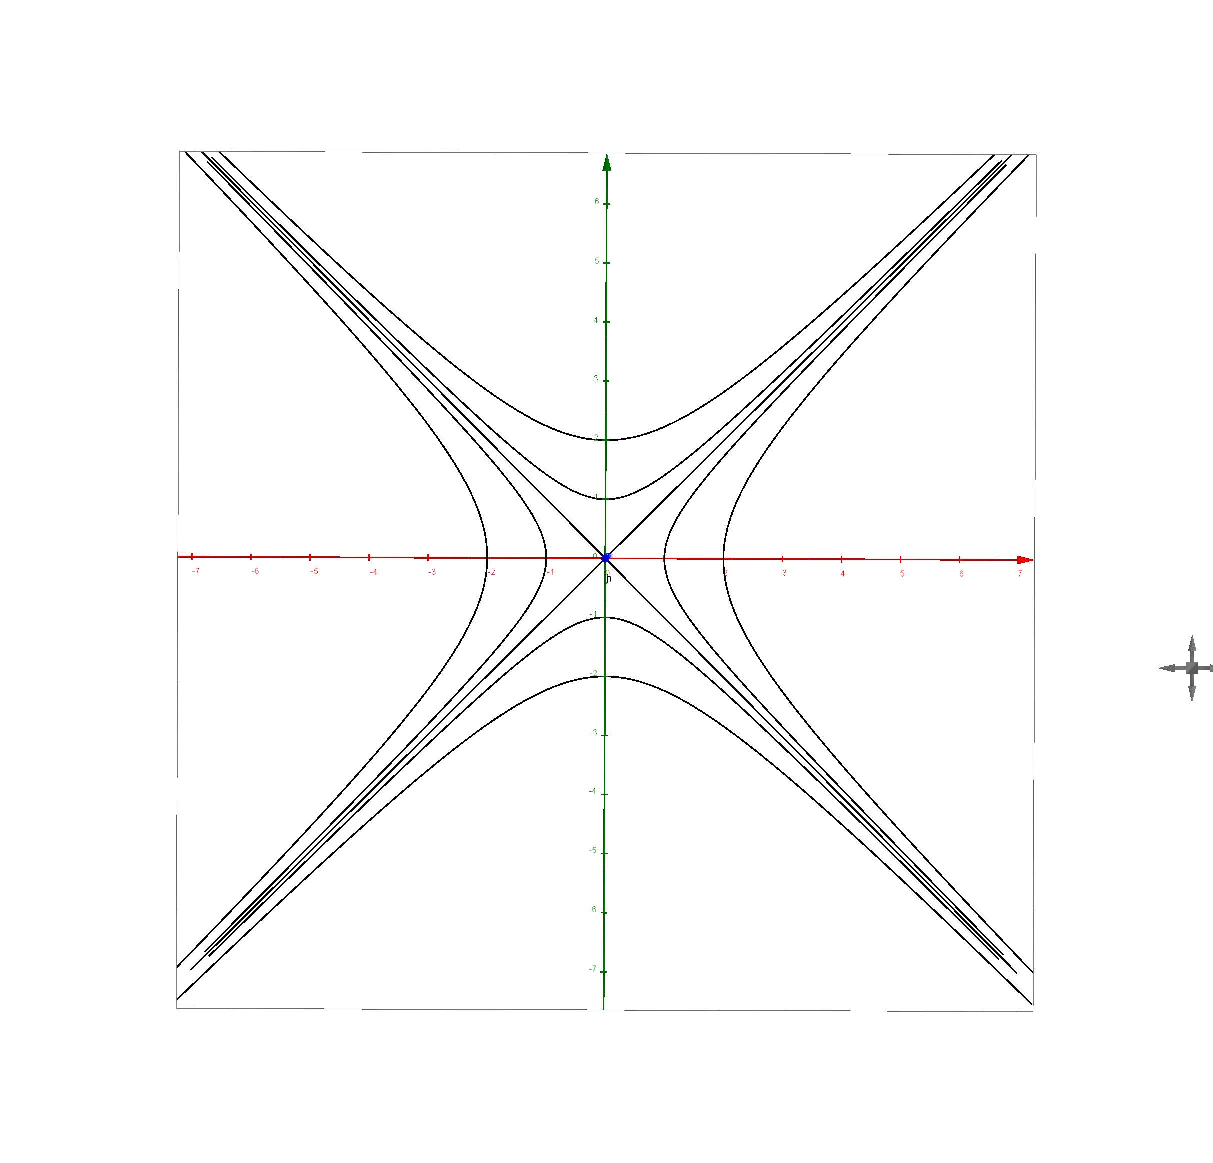
\includegraphics[width=4in]{Hyp_Par}
\end{center}

 \item Sketch the level surface $x^2+y^2-z=4$.

\bigskip

Rearranging, we have the equation $z=x^2+y^2-4$, so the level surface is the graph of the function $f(x,y)=x^2+y^2-4$. Moreover, we recognise this surface as a circular paraboloid, shifted down (in the $z$ direction) by 4 units. Thus, you can obtain your sketch by drawing the standard circular paraboloid (as shown in class) with the origin shifted. If you didn't recognise that the surface is a paraboloid, notice that the sections $x=0$ (in the $yz$-plane) and $y=0$ (in the $xz$-plane) are parabolas with their vertex at $(0,0,4)$, while the section $z=0$ (in the $xy$-plane) is the circle $x^2+y^2=4$. Sketching these three curves gives the following:

\begin{center}
 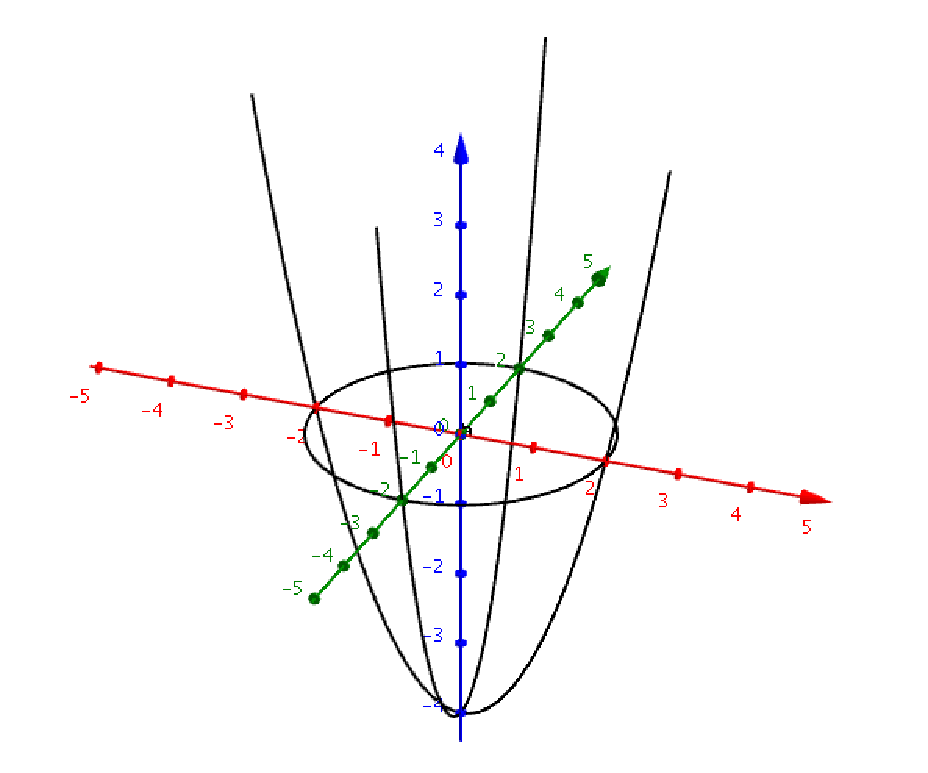
\includegraphics[width=4in]{Paraboloid}
\end{center}

 \item Identify\footnote{That is, tell me if it's a paraboloid, cylinder, hyperboloid, etc.} and sketch the quadric surface defined by the equation $z^2+4y^2=x^2+4$.

\bigskip

We can rearrange this equation as $x^2-4y^2-z^2=-4$. Since all variables are quadradic, and the coefficients don't all have the same sign, we know it has to be a hyperboloid. The only thing that's not clear is whether it's a hyperboloid of one or two sheets. One rule of thumb is that if the constant on the right is positive, the number of minus signs is the number of sheets. Writing the equation as $-x^2+4y^2+z^2=4$ tells us we have a hyperboloid of one sheet. If we know that $z^2+y^2-z^2=c^2$ describes a one-sheeted circular hyperboloid that opens along the $z$-axis, we can guess that this one opens along the $x$-axis, and is elliptical, due the 4 in front of the $y$.

(Note: drawing a hyperboloid opening along the $x$-axis is really hard, if you draw the $x$-axis coming out of the page, as usual. It's easier to re-orient your axes so that the $x$-axis is the vertical axis, and then draw the surface opening vertically.) Below is a computer-generated sketch of the surface in the usual orientation, with several sections shown:
\begin{center}
 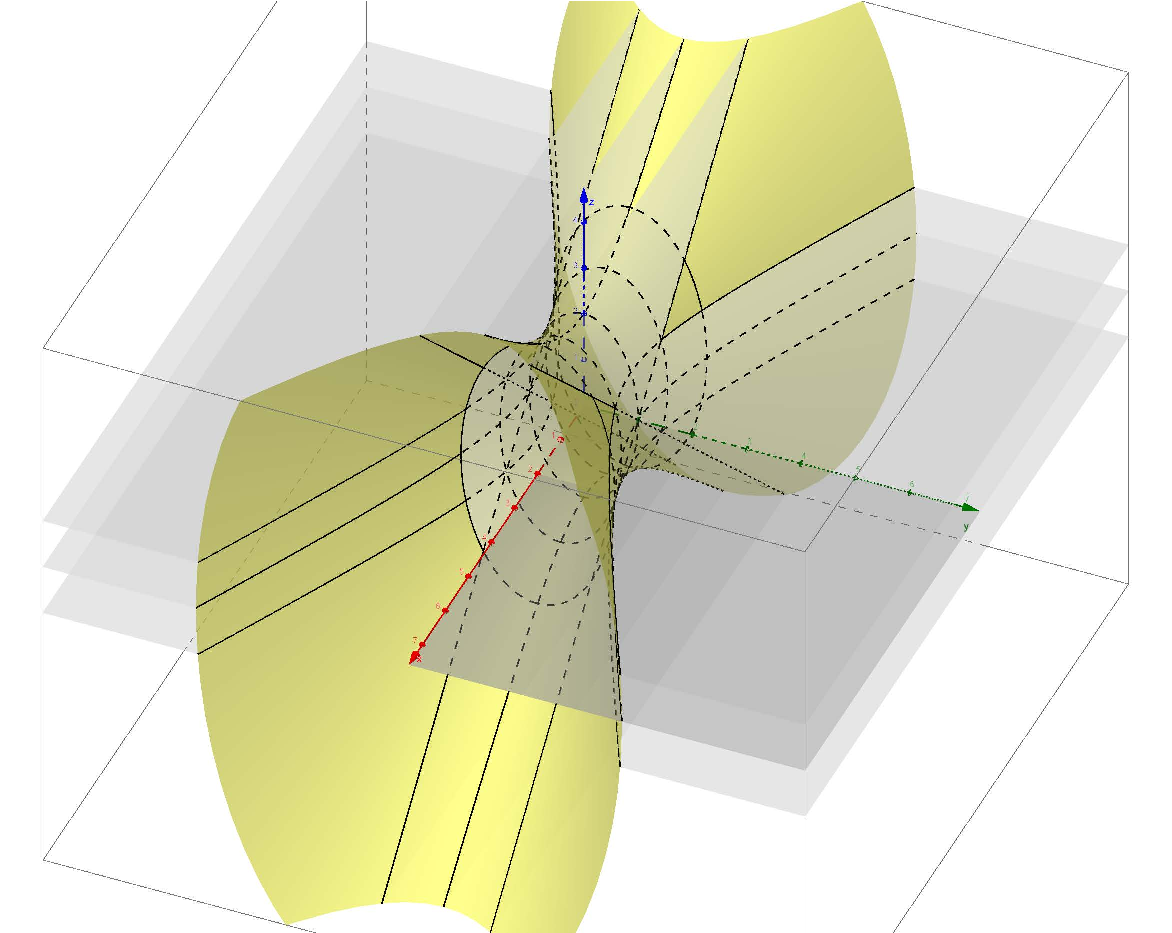
\includegraphics[width=4in]{Hyperboloid}
\end{center}

If you want an interactive version so you can view it from different angles, see\\
 \href{https://tube.geogebra.org/m/A8BBVvd9}{https://tube.geogebra.org/m/A8BBVvd9}.

 \item Show that the intersection of the cone $x^2+y^2=z^2$ and the plane $2z=y+1$ is an ellipse.

\bigskip

There are two approaches to the problem. One is short, but not quite accurate. The other is accurate, but longer. The short approach first:

\medskip

If we solve the equation of the plane for $y$, we have $y=2z-1$. Plugging this into the equation of the cone gives us
\[
 x^2+(2z-1)^2=z^2.
\]
Expanding, we have $x^2+4z^2-4z+1=z^2$, which simplifies to $x^2+3z^2-4z=-1$. If we complete the square in $z$, this becomes
\[
 x^2+3\left(z-\frac{2}{3}\right)^2=\frac{1}{3},
\]
which is the equation of an ellipse. The problem with the solution is that this is the equation of an ellipse in the $xz$-plane, or at best, an elliptical cylinder. It's not too hard to imagine that if we cut such a cylinder by a plane, the result is an ellipse, but this isn't quite a proof.

So what's the longer approach?

\medskip

Writing the equation of the plane as $y-2z=-1$, we note that a normal vector to the plane is $\vec{n}=\langle 0,1,-2\rangle$. Now, we note that the vectors
\[
\vec{u} = \langle 1,0,0\rangle \quad \text{ and } \quad \vec{v} = \frac{1}{\sqrt{5}}\langle 0,2,1\rangle
\]
are unit vectors that are both orthogonal to $\vec{n}$, and also orthogonal to each other. We can use these vectors to define a coordinate system in the plane $2z=y+1$. (Think of $\vec{u}$ and $\vec{v}$ as playing the role of the $\i$ and $\j$ unit vectors in $\R^2$. We want the two vectors to be unit vectors so that an expression like $2\vec{u}+\vec{v}$ can be interpreted as moving 2 units in the $\vec{u}$ direction, and 1 unit in the $\vec{v}$ direction. If the vectors have different lengths, everything will be distorted.)

Setting $x=z=0$ in the equation of the plane, we see that $(0,-1,0)$ is a point on the plane (since $2(0)=(-1)+1$). If $(x,y,z)$ is any other point on the plane, we have the vector equation
\[
 \bbm x\\y\\z\ebm = \bbm 0\\-1\\0\ebm + s\bbm 1\\0\\0\ebm + \frac{t}{\sqrt{5}}\bbm 0\\2\\1\ebm,
\]
where $s$ and $t$ are parameters, which we'll view as coordinates on the plane. (In other words, we can write the vector equation of the plane as $\vec{x} = \vec{x}_0 + s\vec{u}+t\vec{v}$. This equation is telling us that to get to any point on the plane, if we first get to the point $(0,-1,0)$, then we need to travel some distance in the direction of $\vec{u}$, followed by some distance in the direction of $\vec{v}$.)

We can now take the parametric equations $x=s$, $y=-1+\frac{2}{\sqrt{5}}t$, $z=\frac{1}{\sqrt{5}}t$, and plug them into the equation of the cone, giving us
\[
 s^2+\left(-1+\frac{2}{\sqrt{5}}t\right)^2 = \frac{1}{5}t^2.
\]
Expanding, simplifying, and completing the square, the above equation can be rewritten as
\[
 3s^2+\frac{9}{5}\left(t-\frac{2\sqrt{5}}{3}\right)^2=1,
\]
which is the equation of an ellipse in the $(s,t)$-plane, as desired.

{\bf Note:} If you want to go one step further, you can get the parametric equations of the ellipse as a curve in $\R^3$. First, we parameterize the ellipse in the $(s,t)$-plane by setting $s=\dfrac{1}{\sqrt{3}}\cos(u)$ and $t = \dfrac{2\sqrt{5}}{3}+\dfrac{\sqrt{5}}{3}\sin(u)$, for $0\leq u\leq 2\pi$. Using the identity $\cos^u+\sin^u=1$, we can then check (exercise) that $3s^2+\frac{9}{5}(t-2\sqrt{5}/3)^2=1$. Plugging these values into the parametric equations for the plane, we obtain
\begin{align*}
 x &= \frac{1}{\sqrt{3}}\cos(u)\\
 y &= \frac{1}{3}+\frac{2}{3}\sin(u)\\
 z &= \frac{2}{3}+\frac{1}{3}\sin(u)
\end{align*}
You can check that these equations satisfy the equations of both the plane and the cone. If you want to see this curve along with the two surfaces, go to\\ \href{https://tube.geogebra.org/m/BAMdGpnZ}{https://tube.geogebra.org/m/BAMdGpnZ}.

\bigskip


 \item Define the partial derivative $f_z(x,y,z) = \dfrac{\partial f}{\partial z}(x,y,z)$.

\bigskip

Informally, the partial derivative $f_z$ is defined as the derivative that is obtained by treating $x$ and $y$ as constants and differentiating with respect to $z$. Formally, we define
\[
 f_z(x,y,z) = \lim_{h\to 0}\frac{f(x,y,z+h)-f(x,y,z)}{h}.
\]

 \item Compute the partial derivatives $f_x$ and $f_y$ for the function $f(x,y) =e^{xy}\sin(x+y)$ and evaluate them at the point $(0,0)$.

\bigskip

We have
\[
 f_x(x,y) = \frac{\partial}{\partial x}(e^{xy}\sin(x+y)) = ye^{xy}\sin(x+y)+e^{xy}\cos(x+y),
\]
and
\[
 f_y(x,y) = \frac{\partial}{\partial y}(e^{xy}\sin(x+y)) = xe^{xy}\sin(x+y)+e^{xy}\cos(x+y).
\]
Thus, $f_x(0,0) = 0e^0sin(0)+e^0\cos(0)=1$, and $f_y(0,0) = xe^0\sin(0)+e^0\cos(0) = 1$.
 
\end{enumerate}

\end{document}
 
